\cleardoublestylepage{common}

\section{绪论}

\subsection{研究背景与意义}
运动捕捉(Motion Capture)技术也叫做动作捕捉技术,指的是记录生物(多为人体)的运动,并将其使用数学表达,得到描述其三维运动过程的数据。从工作原理上来看,目前的运动捕捉系统主要有以下几种,列举如下:
\begin{description}
    \item[机械式运动捕捉:]这种系统通常由多个关节和刚性的连杆组成,在关节中包含有角度传感器可以测量关节的转动角度的变化。在使用时,通过角度传感器返回的角度值以及已知的各个刚性连杆的长度,就可以计算得到连杆上各端点在空间中的运动情况和位置。这种捕捉系统的优点在于不受环境的影响,精度较高,采样频率也可以达到很高。但是其缺点也是很明显的,该装置使用者佩戴之后动作极其不方便,并且传感器的连杆、线缆等约束了使用者的动作范围。
    % \item[] 声学式的没写 电磁式的没写 
    \item[惯性式运动捕捉:]惯性式动作捕捉系统的核心部分是姿态传感器,此外还有信号接收器与数据处理系统。使用时需要将姿态传感器绑定在肢体的主要部位上,通过无线数据传输方式将姿态信号传送到数据接收器上,然后再进行运动求解。这里的姿态传感器会集成惯性传感器、加速度计、陀螺仪等元素。根据姿态传感器,再结合骨骼的长度信息与骨骼的连接关系,求解出各个关节点的空间位置与运动状态。相比于机械式运动捕捉,惯性式的便携性更强,并且适用范围更广,使用者的动作也几乎不受限制,也能在户外进行使用。但是缺点是其求解位置信息的时候需要将各个部分的运动信息进行积分计算得到位置信息,会造成积分漂移,使得求解出来的位置不准确。
    \begin{figure}[ht] \centering
        \subfigure[惯性式运动捕捉系统] {
        \includegraphics[height=0.25\columnwidth]{figure/background/imu}
        }
        \subfigure[标记点光学式运动捕捉系统(图源\cite{lingyun})] {
        \includegraphics[height=0.25\columnwidth]{figure/background/lingyun}
        }
        \caption{运动捕捉系统}
        \label{fig:motion}
    \end{figure} 
    \item[标记点光学式运动捕捉:]光学式动作捕捉系统是目前电影制作工业常用的方法之一,一般会在人体运动的关键地方粘贴标记点(Markers),然后使用多个相机从不同的角度实时检测人体身上的标记点,根据三角测量原理计算标记点的空间坐标,再解算出人体的哥哥骨骼的6自由度的运动。这种方法标记点的佩戴就更为方便了,并且运动也基本不受限制。但是其对拍摄环境的要求较高,人体身上的标记点也容易混淆,需要人工在后期进行处理。同时,拍摄的人也无法穿着日常的服装,需要被拍摄人穿着紧身服装,以及在服装上贴上标记。例如,国内的凌云\cite{lingyun}的全身运动捕捉系统,如图\ref{fig:motion}(b)所示,采用了850nm红外光源照明捕捉精度即可高达0.1mm。 
    \item[无标记点运动捕捉:]这种方法只需要输入普通的视频图像,就可以进行运动捕捉,通过对二维图像上的人体关节点位置进行检测,再根据多相机的位置计算关节的三维坐标,即可进行恢复。对使用者基本不需要任何额外的标记物,也不需要佩戴任何传感器,对使用者的衣着也没有要求,可以适用于较大范围的场景。其缺点是相对于上述的方法来说精度较低。因此在对精度要求不是特别高的场景下,可以采取牺牲精度的方法来换取更高的适应能力。本文的主要研究内容即是这一类方法。
\end{description}

人体运动捕捉技术涉及到了计算机视觉领域的许多基本问题。例如运动检测技术、物体识别或人体识别技术、多摄像机数据融合。这一项技术还融合了其他方向的技术,例如图像处理技术、计算机图形学的技术、人体运动学以及优化理论,具有较高挑战性。同时,该技术拥有着广泛的应用场景,例如在智能监控中对人体的姿势和行为进行跟踪分析,在进行人机交互时对人的身体姿势与动作的识别,以及在动画和影视行业里人物动作的捕捉。
基于视频的人体运动姿态分析有着广阔的引用场景,因此其吸引了越来越多研究者的兴趣。其应用领域主要表现在以下几个方面:

\begin{figure}[ht] \centering
    \subfigure[AR场景] { \label{fig:a}
    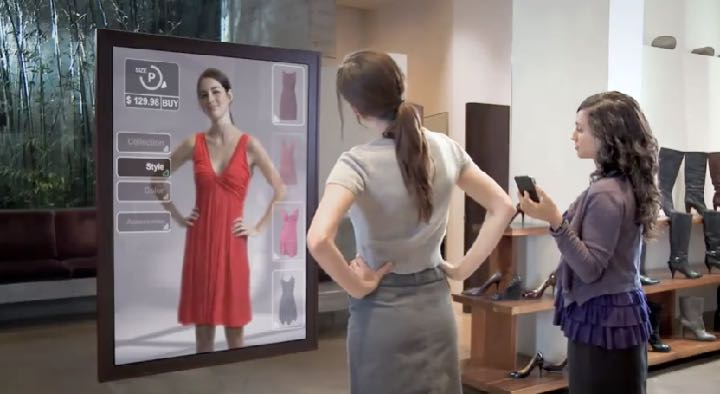
\includegraphics[height=0.15\columnwidth]{figure/background/ar.png}
    }
    \subfigure[人机交互] { \label{fig:appb}
    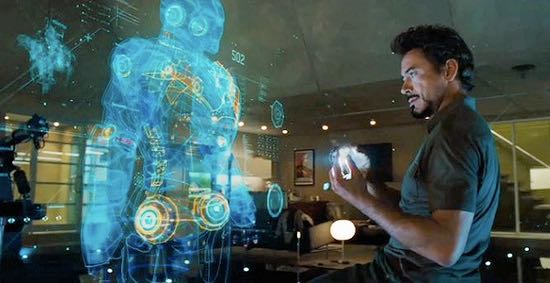
\includegraphics[height=0.15\columnwidth]{figure/background/hcl.png}
    }
    \subfigure[电影制作] { \label{fig:appc}
    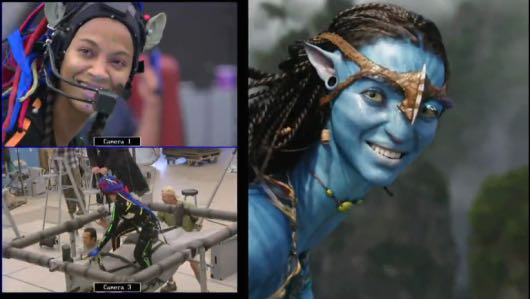
\includegraphics[height=0.15\columnwidth]{figure/background/movie.png}
    }
    \subfigure[娱乐游戏] { \label{fig:appd}
    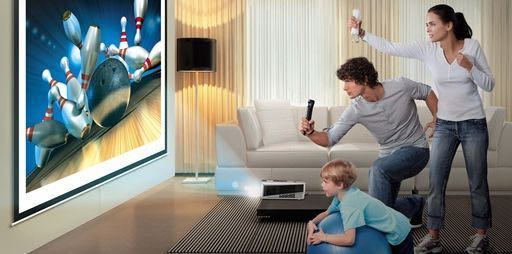
\includegraphics[height=0.15\columnwidth]{figure/background/gaming.png}
    }
    \subfigure[健康监护] { \label{fig:appe}
    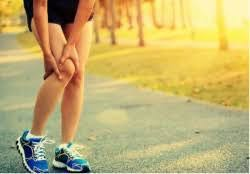
\includegraphics[height=0.15\columnwidth]{figure/background/health.png}
    }
    \subfigure[安防监控] { \label{fig:appf}
    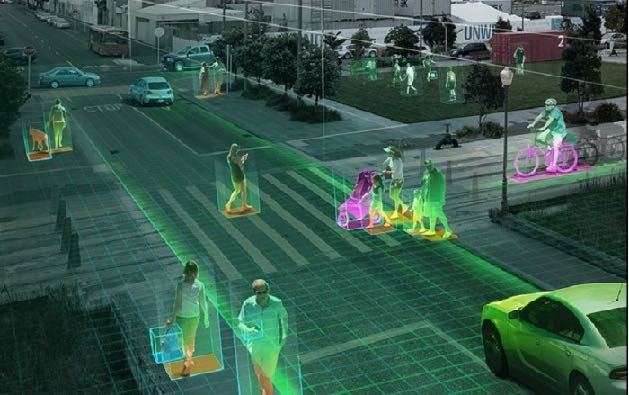
\includegraphics[height=0.15\columnwidth]{figure/background/surveil.png}
    }
    \caption{应用场景}
    \label{fig:appli}
\end{figure}


\textbf{虚拟现实和增强现实:}在虚拟环境中,人与虚拟角色进行的动作模拟,可以通过基于视频的人体姿态运动分析,给参与者提供更多的交互形式。计算机可以从视频中获取人体运动数据,可以使我们用新的虚拟人物或者动画角色替换原始视频中的人物,得到更好的效果。

\textbf{智能人机交互:}智能人机交互是指让目前的计算机摆脱键盘鼠标等传统交互设备的局限,通过人体运动等更为自然的方式直接用人类进行交互,使得计算机能像人与人之间的交流一样更自然便捷。这要求计算机能够更进一步地从面部表情、语言、身体动作去分析人的行为,而基于视觉分析的技术能够在语言干扰大的环境下提供更准确的输入。

\textbf{电影制作:}基于视频的人体运动动作的获取,将给人体动画和游戏提供更加丰富的数据,并且也能大大降低运动捕捉系统的成本,提高制作效率。

\textbf{健康监护:}在临床上,通过获取患者的行走动作,利用计算机来分析其运动数据,有助于判断身体某部分的受伤情况或者畸形程度,从而帮助做出有效的治疗手段。而传统的运动分析系统大多采样专用的视频设备和计算机设备,价格昂贵,操作复杂,使用过程具有较高的专业性,因此不适合进行大范围的推广,难以在普通医院使用。因此采用普通电脑连接普通摄像机的人体运动姿态分析系统有着更广阔的应用场合和前景。

\textbf{智能安防监控:}目前监控摄像机在公共场所已经广泛存在,但是无法发挥其实时、积极的作用,大多数场合只能通过专门的工作人员监视显示器,以发现异常的事件。或者将监控视频保存,出现异常情况时,才调用监控记录进行查看,而这样又会占用大量存储设备,因此无法保留长时间记录。如果通过视频进行监视,通过计算机进行实时分析,通过检测并跟踪其中的人体运动,分析人体行为,当有异常情况发生时,系统能够及时警报,从而有效防止此类事件的发生。同时也可以减少大量雇佣人员的成本,以及购买存储设备的成本。

\subsection{LightStage系统}
基于多个视频序列的运动捕捉系统一般会使用摄像机阵列,从不同的角度同时拍摄不同视角下的图像。摄像机阵列系统通常是由相机阵列、辅助光源组成,相机通过信号进行同步控制,拍摄同步的图片。而不同的相机阵列包含的相机数目也不同。目前世界上学术界比较知名的的摄像机阵列系统有卡耐基梅隆大学的Panoptic Studio系统。国内的有清华大学的Multi-Camera Dome系统,以及浙江大学的人体反射场高速获取系统,即本文所使用的运动捕捉系统,以下称为LightStage 系统。

卡耐基梅隆大学的Panoptic Studion系统\cite{Panoptic}如图\ref{fig:panoptic}所示,该系统的主要硬件为:(1)480个VGA相机,其分辨率为640x480,帧率为25帧每秒,这些相机通过硬件的时钟来进行同步;(2)31个高清相机,其分辨率为1920x1080,帧率为每秒30帧,这些相机也是通过硬件时钟来进行同步的。(3)10个Kinect传感器这些传感器能够提供\(1920\times 1080\)的三通道彩色图片,以及512x424的深度图片,帧率为每秒30帧。这个系统的主体是一个半球形的结构,主要用于拍摄多人社交场景、恢复出视频中的人体姿态等。

\begin{figure}[ht] \centering
    \subfigure[结构图\cite{Panoptic}] {
    \includegraphics[height=0.25\columnwidth]{figure/background/panoptic}
    }
    \subfigure[Panoptic数据集样例\cite{Panoptic}] {
    \includegraphics[height=0.25\columnwidth]{figure/background/bang}
    }
    \caption{\label{fig:panoptic} Panoptic Studio示意图\cite{Panoptic}}
\end{figure} 

目前该数据集开源了65个视频序列,总共5.5小时,其中包含了150万的人体骨架数据。可以使用的数据有通过480个相机恢复出来的人体骨架数据、人体脸部关键点的三维数据、人体手部关键点的数据。该系统在进行所有的521个相机的标定的时候,采用的方法是运动恢复结构(Structure from Motion)的方法。该方法的主要流程是通过检测场景中的特征点,对不同视角下的特征点进行匹配,然后估计出各个相机的位置。他们使用了开源软件VisualSfM进行重建,整个相机标定过程用了6个场景,标定需要12小时的时间。

浙江大学的人体反射场高速获取系统位于浙江大学紫金港校区蒙民伟楼。该系统的主要组成部分是24个RGB图像同步摄像机,相机能够拍摄得到分辨率是\(2048\times 2048\)的高清视频,拍摄的视频帧率可控,最高可以达到50帧每秒。24个相机均匀布置在框架上,环绕成一圈;系统的框架部分,整个系统是一个半球形的钢架结构,直径长达7m;系统的灯光部分,整个半球形的结构上分布着近1000盏LED冷光灯,灯光以9个为一组,每一组的开断与灯光的闪烁频率均可使用程序控制。如图\ref{fig:lightstage}所示。
\begin{figure}[htbp]
    \centering
    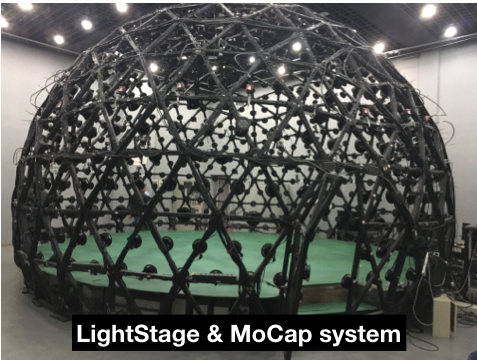
\includegraphics[width=0.6\linewidth]{figure/background/lightstage}
    \caption{\label{fig:lightstage} 浙江大学人体反射场高速获取系统}
\end{figure}

\subsection{国内外研究现状}

对于三维人体姿态估计问题,目前的方法主要分为两类:端到端法(end-to-end)\cite{pavlakos2017coarse}和两步法(two-step)\cite{zhou2016sparseness}。端到端法(end-to-end)\cite{pavlakos2017coarse}是指对输入的图像或者视频通过一个卷积网络(ConvNet)的处理直接得到人体的三维姿态;而两步法(two-step)\cite{zhou2016sparseness}通常是指先根据输入的图像或视频,提取出对应的二维人体姿态,再使用优化的方法或神经网络的方法得到人体的三维姿态。

三维人体姿态估计问题,从相机的数量来分又可以分为单目(single-view)三维人体姿态估计和多目(multi-view)三维人体姿态估计。相比于单目的人体姿态估计,多目的方法可以利用多个视角的额外信息,从而从中提取出更为准确的三维人体姿态,消除单个所带来的深度的不确定性。

从估计的人数上来分,三维人体姿态估计又可以分为单人(single-person)三维人体姿态估计和多人(multi-person)三维人体姿态估计,多人的姿态估计问题相比单人的更加复杂,多人之间的人体互相遮挡与交叉的情况更多,因此也是当前研究的热点所在。

\subsubsection{二维人体姿态估计}
二维人体姿态估计问题,就是从输入图像或视频中,得到在图片上人体的关节点的位置。传统的人体姿态估计的方法对人体结构进行建模,将人体部位的空间相关性用一个树型结构图表示(tree-structured graphical model)\cite{eichner20122d}。近些年来,深度卷积网络(ConvNet)在二维人体姿态估计问题中取得了重大的进展。早期使用卷积网络(ConvNet)的方法,直接预测人体关节点的坐标\cite{toshev2014deep},如\refFig{fig:deeppose}所示,这种方式想法直接,但是实际效果并不好。后来人们采用回归热图(heatmaps)\cite{pfister2015flowing}的方案,来间接预测人体关节点,如\refFig{fig:heatmap}所示。这种方法更适合于卷积网络,它首先在图像上为每个关节点回归一个热图,然后再从中提取出关节点的位置。与直接预测相比,预测热图有以下优点:首先,它避免使用卷积网络来直接预测实际值的问题;其次,它可以处理图像中有多个实例的问题。
\begin{figure}[ht]
    % 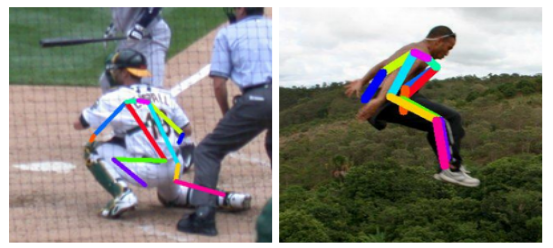
\includegraphics[width=0.32\linewidth]{review/deeppose.png} \hfill
    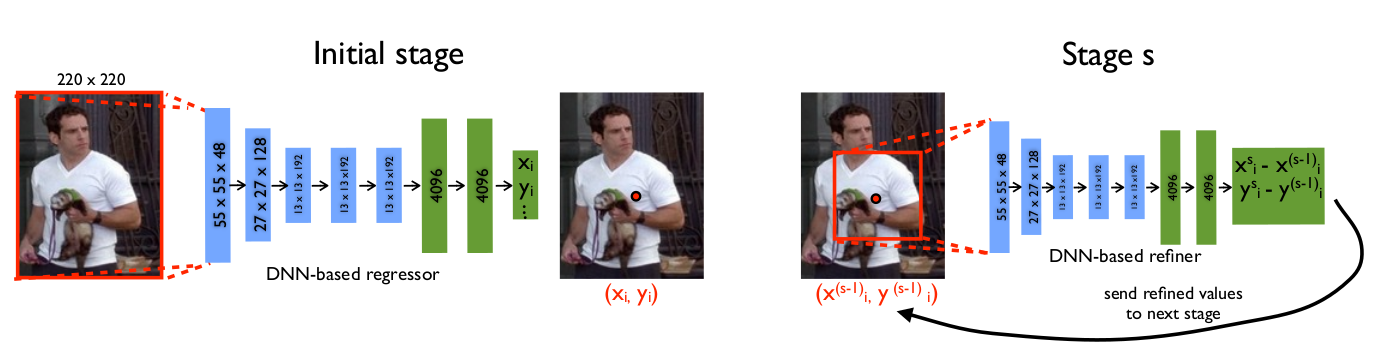
\includegraphics[width=1\linewidth]{review/deeppose_line.png}
    \caption{Deeppose方法\cite{toshev2014deep}:基于深度神经网络对人体姿态进行回归。左:网络结构可视化,其中蓝色表示卷积层,绿色表示全连接层;右:使用上一阶段的结果取出原图的的部分,对结果进行优化。}\label{fig:deeppose}
\end{figure}

\begin{figure}[ht]
    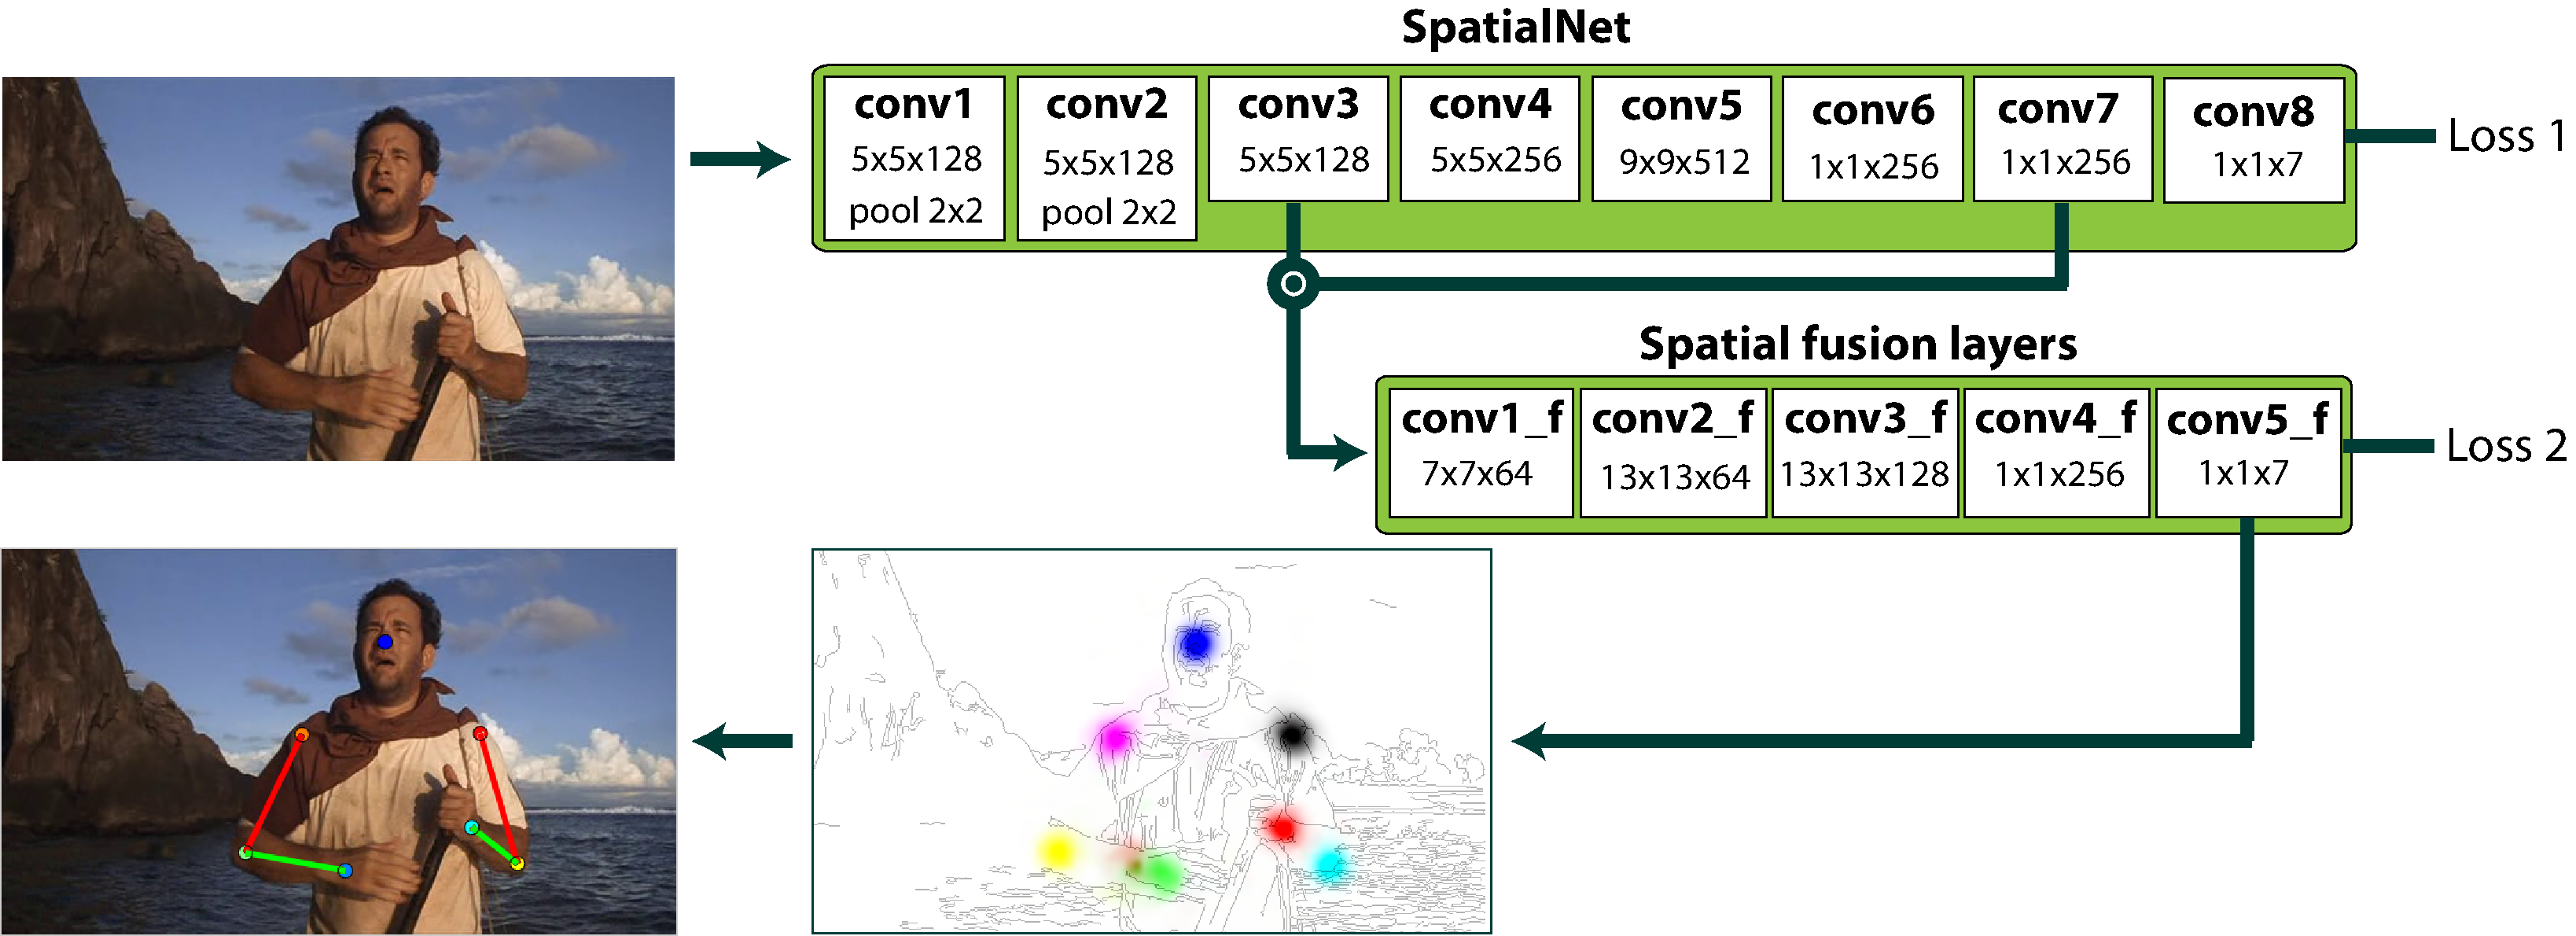
\includegraphics[width=1\linewidth]{review/heatmap.pdf}
    \caption{回归热图\cite{pfister2015flowing}:对于每一个关节,网络的学习目标是一个热图(heatmap),每个关节的热图是根据关节的真实位置生成的一个高斯分布。同时还通过在不同层次上的特征的混合,使网络学到一个隐式的空间模型。}\label{fig:heatmap}
\end{figure}

在此之后,研究者们设计了许多不同的网络结构,在这一问题上取得了非常好的效果,例如卷积姿势机(Convolutional Pose Machines),堆叠沙漏网络(Stacked Hourglass Networks)\cite{newell2016stacked}。2016年,Stacked Hourglass网络\cite{newell2016stacked}被提出,如\refFig{fig:hourglass}所示。这种网络与之前的结构完全不同,它采用重复的自底向上和自顶向下的漏斗形,并且在中间加入了监督。这样能够利用多个尺度的信息来猜测被遮挡关节的位置,能比级联的效果更好。而之后的很多三维姿态的研究,都是基于这个网络做的。

\begin{figure}[ht]
    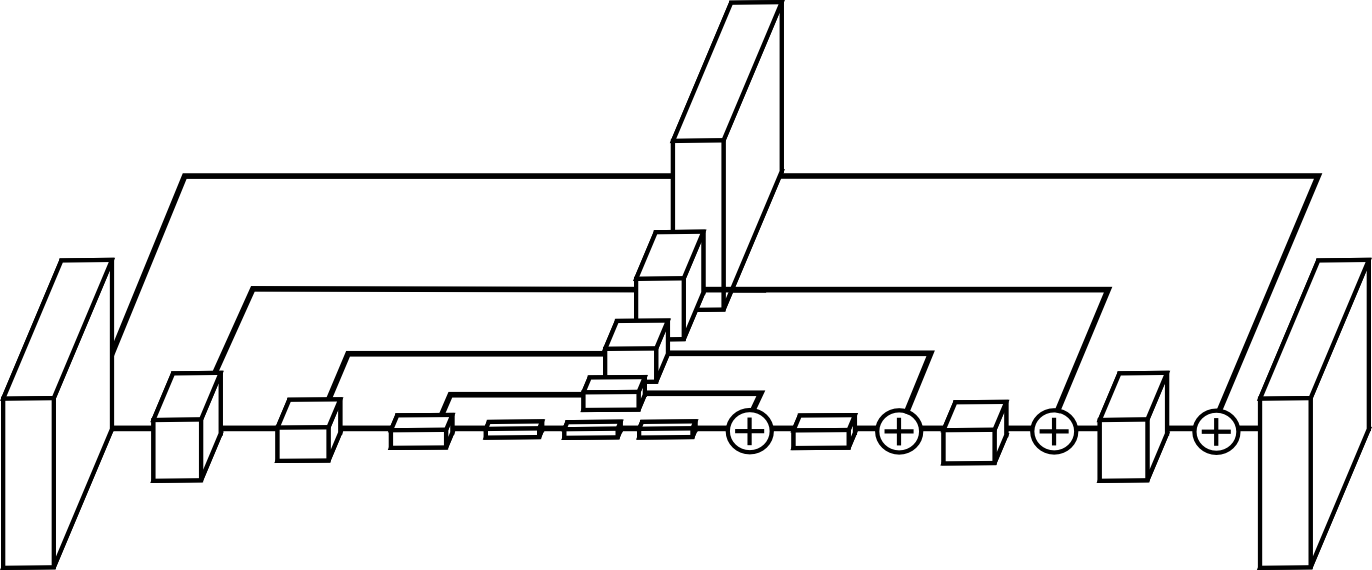
\includegraphics[width=0.4\linewidth]{review/single-hourglass.png}
    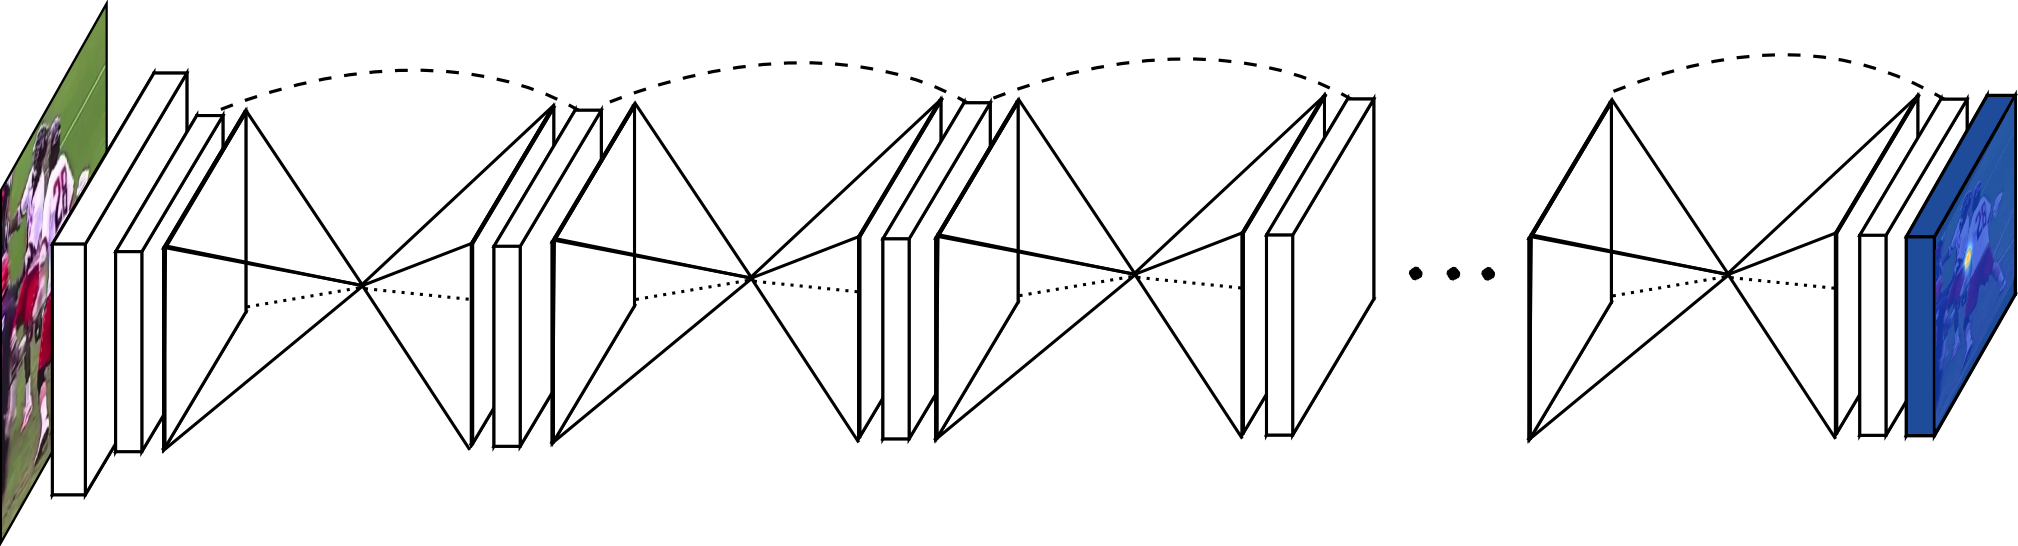
\includegraphics[width=0.59\linewidth]{review/stacked-hg.png}
    \caption{堆叠沙漏网络\cite{newell2016stacked}:左:单个沙漏网络。使用了连续的下采样与上采样,并将不同步骤的信息混合起来。右:多个沙漏网络串联在一起,能够不断利用前一步的网络输出进行优化}\label{fig:hourglass}
\end{figure}


\subsubsection{三维人体姿态估计}
目前大部分论文将三维人体姿态估计问题作为从图像或视频中得到人体的主要的关节点的空间位置问题。在这种定义下,三维人体的姿态估计方法可以分为两类:两步法和端到端法。

两步法的主要流程如下:第一步获取人体的二维关节点位置;第二步,从三维动作捕捉的数据集上学习得到人体骨架的先验知识,例如学习一个姿态字典\cite{zhou2015sparse},如\refFig{fig:twostep}所示。由于从二维到三维的估计具有不确定性,这些方法对四肢长度或骨架的尺寸比例进行假设,作为先验知识。两步法的优点是对不同场景的图片更为鲁棒,而且只需要二维动作与三维动作配对的数据集,不需要有图像配对的三维姿态数据集。该方法的缺点是较为依赖二维关节点的检测,在估计二维关节点时如果出错的话恢复出的三维关节点效果就会较差。

\begin{figure}[ht]
    \centering
    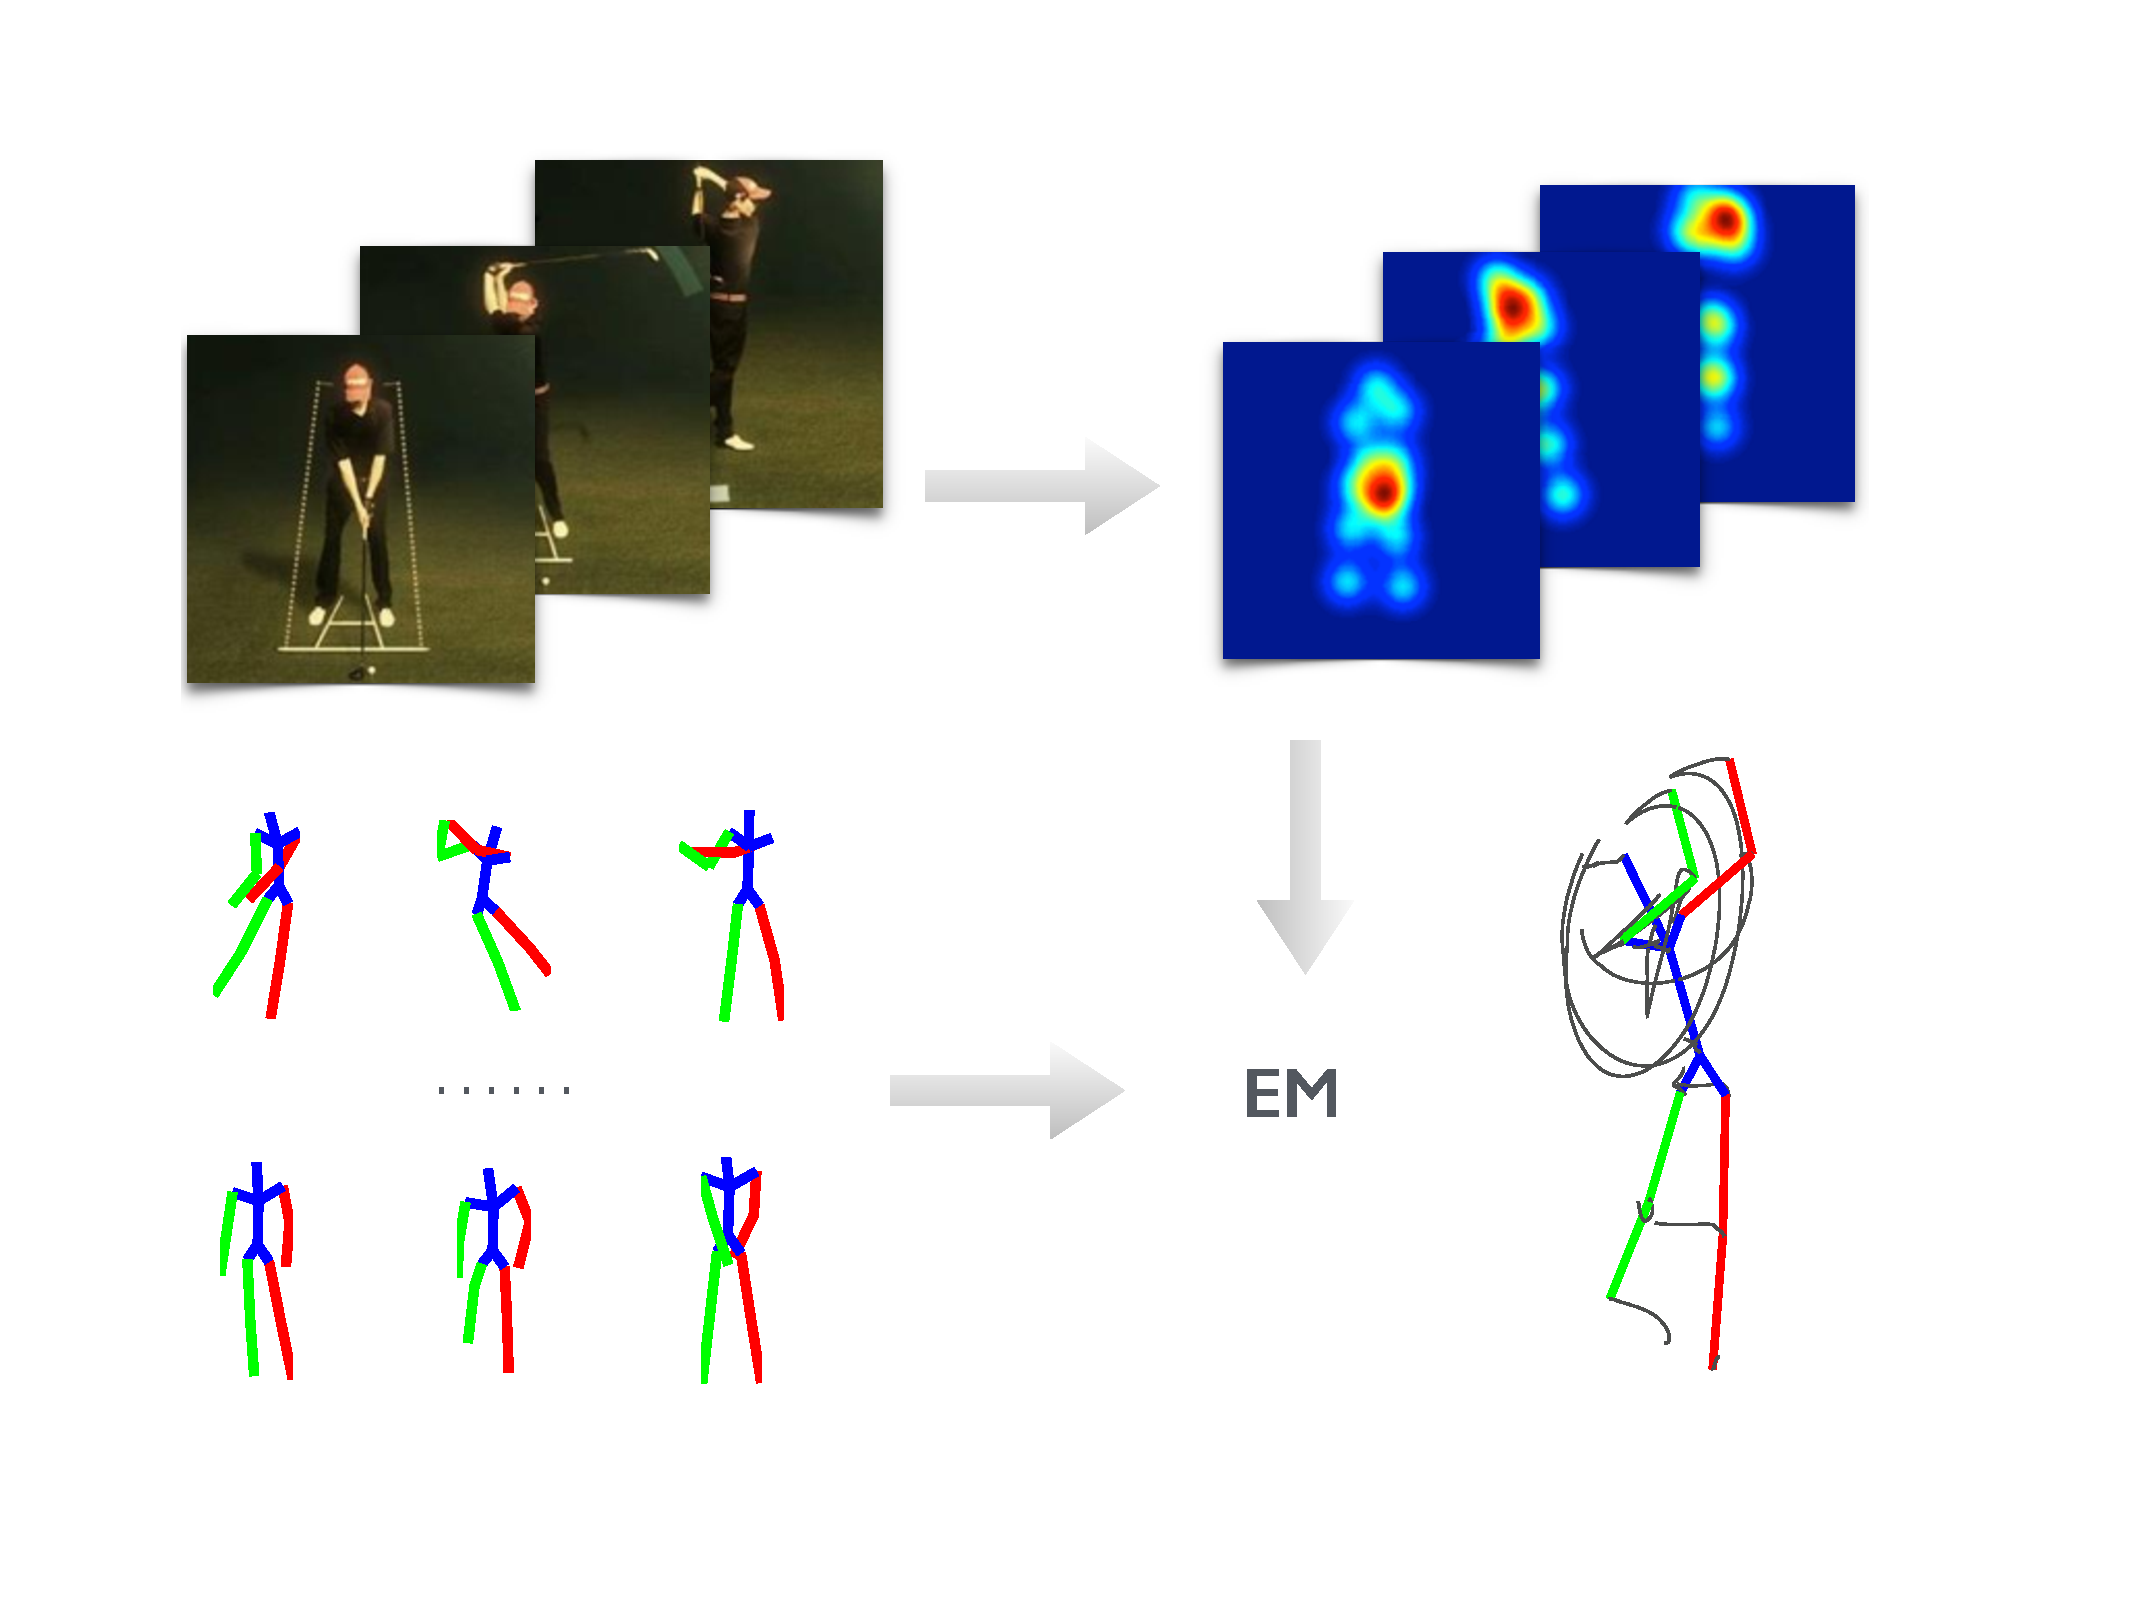
\includegraphics[width=0.4\linewidth]{figures/overview.pdf}
    \caption{两步法\cite{zhou2015sparse}:先从图片中得到人体的二维姿态,再从二维姿态中恢复三维姿态}\label{fig:twostep}
\end{figure}

从 Toshev \cite{toshev2014deep}等人开始,最近的许多文献的方法都是在深度学习框架下直接从输入图像估计得到三维关节点\cite{pavlakos2017coarse,zhou2017weaklysupervised}。%Rogez\cite{rogez2016mocap}等人将人体检测与 3D 人体姿态估计相结合。
这种端到端法(end-to-end)的优点如下:能够充分利用输入图像的信息,训练过程简单不需要像两步法(two-step)那样先进行 2D 人体姿态估计,再进行后续处理。但是该方法的缺点也是比较明显的,之前所说的这些直接估计的方法的所使用的具有准确的三维标注的图像均是在受控的动作捕捉系统中捕获。仅在这些受控环境数据集上训练的模型不能很好地泛化到现实世界。

\begin{figure}[ht]
    \centering
    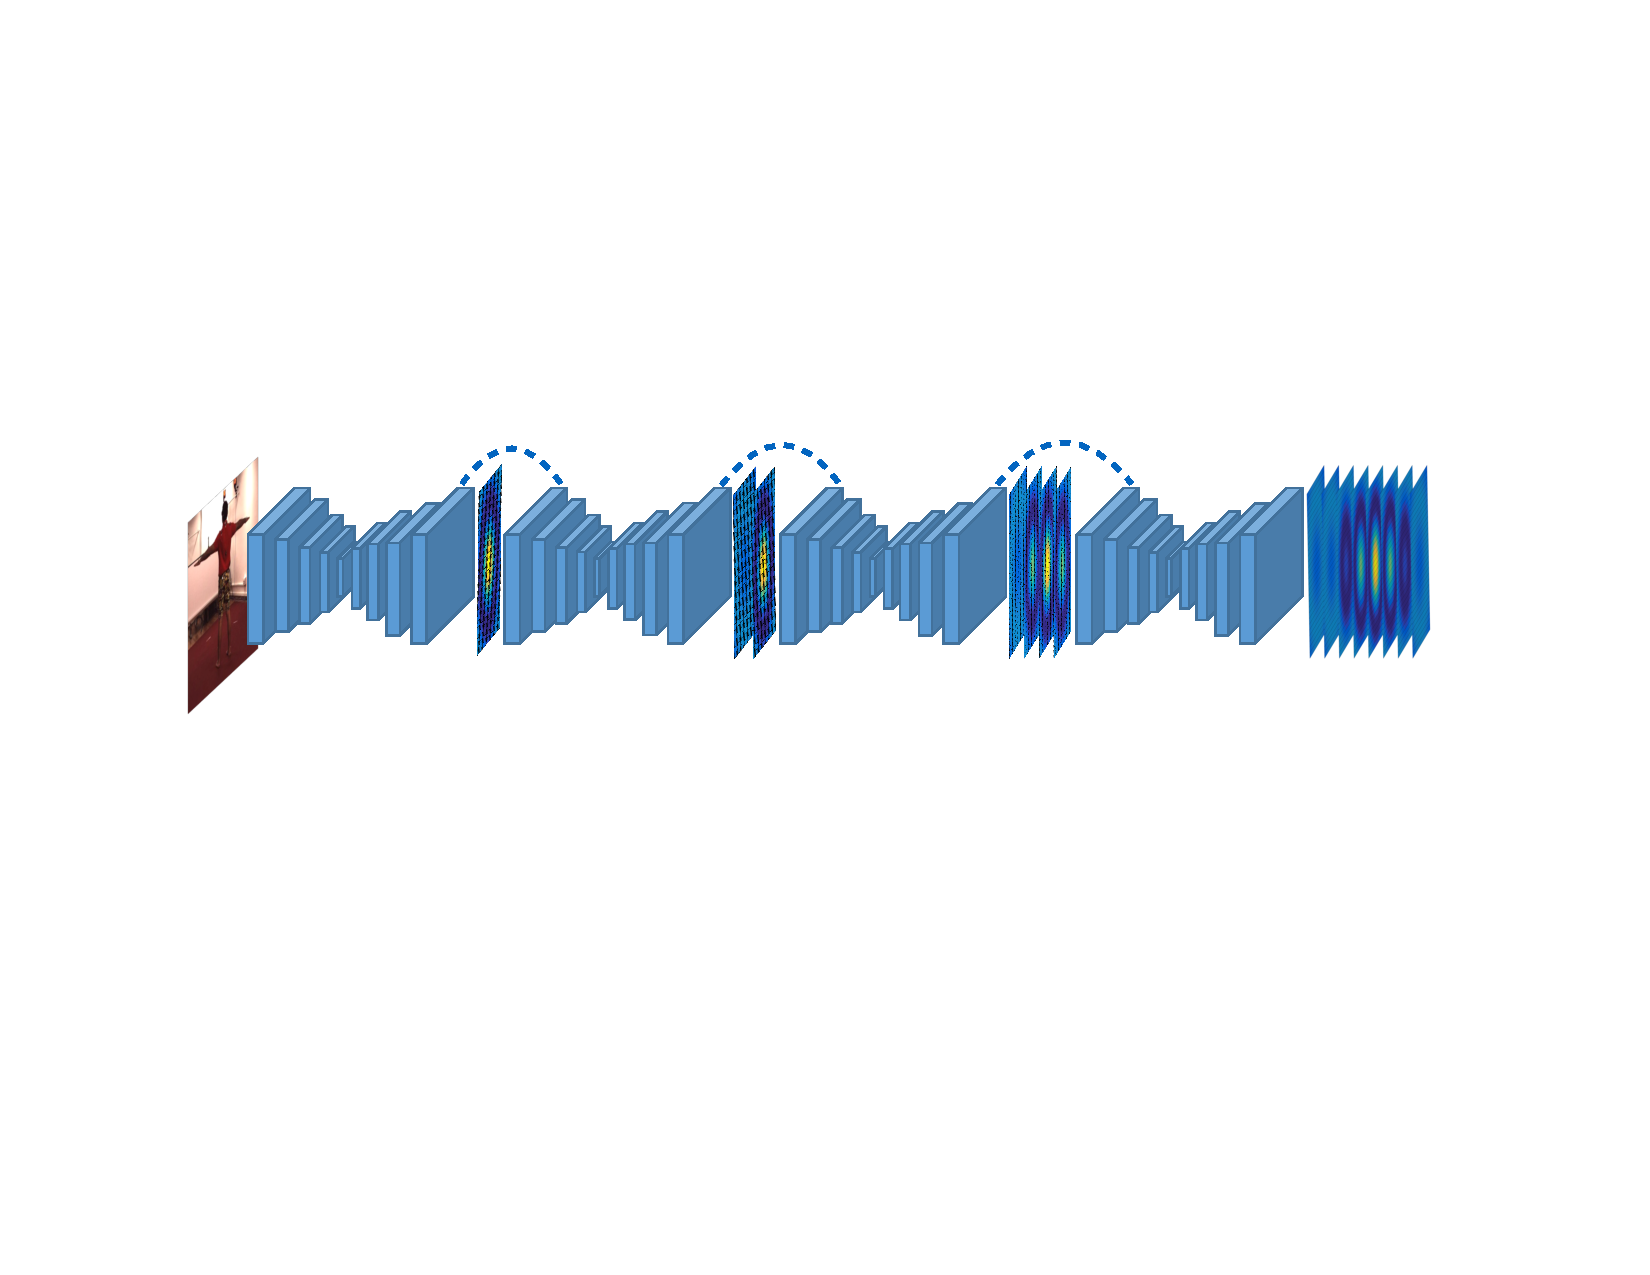
\includegraphics[width=1\linewidth,trim={2.7cm 9.5cm 3.5cm 7.4cm},clip]{review/coarse-to-fine.pdf}
    \caption{由粗到细\cite{pavlakos2017coarse}:从输入图片中去估计每个关节的深度,深度方向的分辨率由粗到细}\label{fig:c2f}
\end{figure}

当下有一些文献认为仅仅用 3D 骨架的方法来描述 3D 姿态过于简单, Bogo等人\cite{bogo2016keep}提出了 SMPLify,一种基于优化的,从 14 个检测到的二维关节恢复SMPL 参数的方法。SMPL\cite{loper2015smpl}是一种参数化表示的人体模型,这个模型从大量三维人体扫描数据中去学习人体的参数化表示,使得人们可以通过低维的参数去表示不通形状的人体模型。Bogo等人\cite{bogo2016keep}使用了优化的方法,将人体模型拟合到从图片中检测出来的二维人体关键点上。但是,由于加入了优化步骤,该方法不是实时的,每个图像需要 20-60 秒的时间进行处理。同时,由于从二维到三维的歧义性,他们在优化过程中加入了许多先验的知识,例如关节的角度的旋转范围,以及一个大量的姿势数据,使得得到的姿势接近数据库中的姿势。其部分结果如\refFig{fig:smpl1}所示。 

\begin{figure}[ht]
    \centering
    \includegraphics[width=0.8\linewidth]{review/smplify.pdf}
    \caption{Keep it SMPLify\cite{bogo2016keep}:通过拟合SMPL人体模型到图片的二维关键点上}\label{fig:smpl1}
\end{figure}

Lassner \cite{lassner2017unite} 等人 从 SMPLify 的结果训练 91 个关键点探测器,其中一些相当于传统的身体关节,其他对应于身体表面的位置。然后,他们优化SMPL 模型参数以适应与\cite{bogo2016keep}类似的关键点。他们还提出了一种随机森林回归方法来直接回归 SMPL 参数,从而以精确性为代价减少运行时间,如\refFig{fig:up}所示。而近期Kanazawa 等人\cite{kanazawa2018end} 的方法直接从图像推断 SMPL 参数,而不依赖于检测到的 2D关键点,并且做到了实时运行。

\begin{figure}[ht]
    \centering
    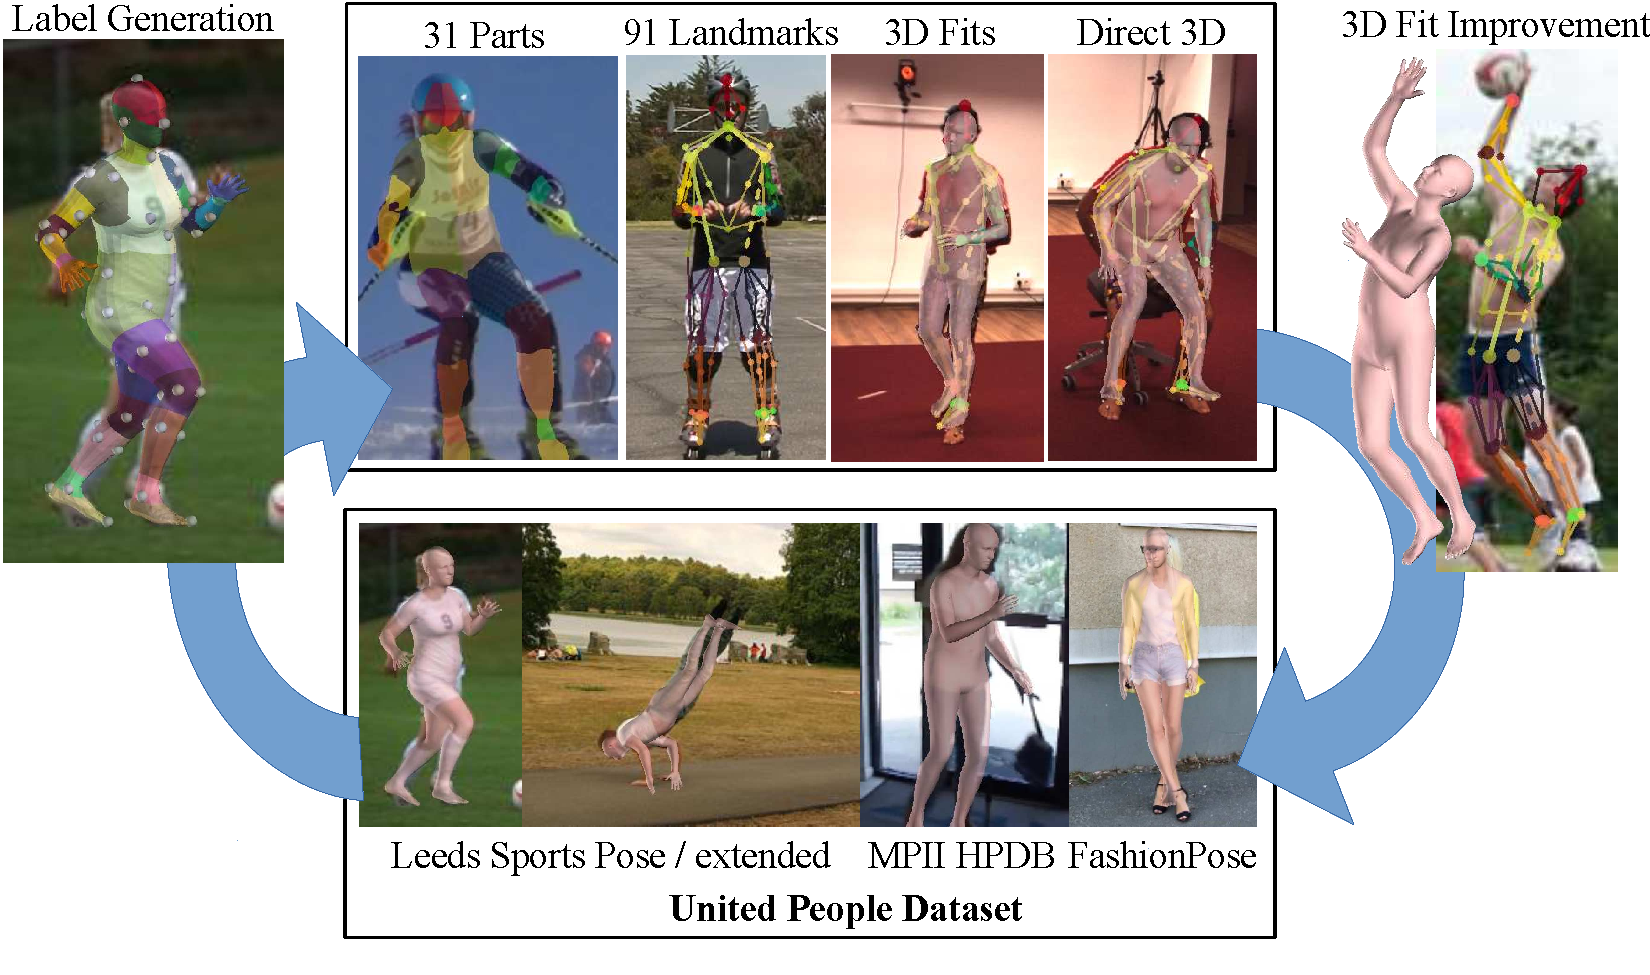
\includegraphics[width=0.8\linewidth]{review/up.pdf}
    \caption{Unit the people\cite{lassner2017unite}:通过拟合SMPL模型到检测的人体的91个关节点上}\label{fig:up}
\end{figure}

\subsection{本文的主要工作和贡献}

本文旨在提出针对光场系统同步高速采集的视频序列进行自动人体三维重建的软件系统,这个系统涵盖了多视角三维重建的各个阶段。该系统的硬件平台为浙江大学CAD\&CG国家重点实验室所搭建的人体反射场高性能采集系统,以下简称Light Stage系统,通过该平台我们能够采集得到同步的相机阵列视频序列,以采集的数据为基础,我们完成了一套稳定并且鲁棒的自动人体三维重建软件,主要包括了相机标定、颜色校正、人体二维关节点检测、人体三维关节点重建、人体几何模型重建等步骤。不仅能够从单目相机的数据中获得人体的二维关节点位置结果,还能充分利用该平台的多视角的同步特性,综合考虑多视角的几何信息,使得重建的结果更加鲁棒。在此基础上,还对人体几何模型进行了拟合,对人体的各个关节的三自由度进行了估计,有效地捕获了人体的运动过程,能够较好的满足在运动捕捉、电影处理、虚拟现实等相关应用的需求。

\subsection{本章小结}
本章首先介绍了运动捕捉系统的发展现状以及常用的各种运动捕捉系统方法,并对其各自的优点与缺点进行了介绍,并阐述了基于视频的运动捕捉方法的优势与不足之处。接着介绍了本文的研究所基于的硬件平台,并对基于视频的人体姿态估计的国内外研究现状进行了介绍,主要介绍了本文所涉及到的二维人体关节点检测技术、三维人体关节点检测技术、人体几何模型表示技术的发展现状。最后介绍了本文的主要研究内容和贡献。

本文接下来的组织按照本文项目的不同模块进行展开:在第二章,首先介绍了利用深度神经网络方法进行的人体二维关节点检测的三种方法,进行人体二维关节点的检测,展示了其检测结果,并在开源数据集上进行了定量的实验,对三种方法进行了量化分析;在第三章,介绍了如何在多摄像机阵列下进行人体三维关键点重建,从摄像机阵列的标定开始,以及利用方程求解的方法与最优化的方法进行求解;在第四章,引入了人体三维几何模型,使用最优化的方法进行人体的各关节的六自由度的恢复,得到具有表现力的模型;在第五章中,对本文所做的工作进行了总结,并对未来的工作提出展望。
